\documentclass[12pt]{article} % JASA requires 12 pt font for manuscripts

\usepackage{afterpage} % for better control of the floats

%\usepackage{endfloat} % just for while I am writing

% for citations
\usepackage[authoryear]{natbib} % natbib required for JASA
% \usepackage[colorlinks=true, citecolor=blue, linkcolor=blue]{hyperref} % comment out and use url package for submission

% for the fancy tables with the icons
%\usepackage[margin=1.0in]{geometry}% http://ctan.org/pkg/margin
\usepackage{booktabs}% http://ctan.org/pkg/booktabs
\usepackage{array}% http://ctan.org/pkg/array
\newcolumntype{M}{>{\centering\arraybackslash}m{\dimexpr.05\linewidth-2\tabcolsep}}



\usepackage[usenames,dvipsnames]{xcolor}


%\definecolor{Blue}{rgb}{0,0,0.5}
\newcommand{\hh}[1]{{\color{magenta} #1}}
\newcommand{\al}[1]{{\color{ForestGreen} #1}}

\newcolumntype{C}[1]{>{\centering}m{#1}}
% fonts
%\usepackage{kpfonts}

% for figures
\usepackage{graphicx,psfrag,epsf}
\usepackage{enumerate}
\usepackage{natbib}
\usepackage{url} % not crucial - just used below for the URL 

\graphicspath{{figure/}}


%\pdfminorversion=4
% NOTE: To produce blinded version, replace "0" with "1" below.
\newcommand{\blind}{0}

% DON'T change margins - should be 1 inch all around.
\addtolength{\oddsidemargin}{-.5in}%
\addtolength{\evensidemargin}{-.5in}%
\addtolength{\textwidth}{1in}%
\addtolength{\textheight}{1.3in}%
\addtolength{\topmargin}{-.8in}%


\usepackage{wrapfig,float}
\usepackage{caption}
\usepackage{subcaption}

% help with editing and coauthoring
\usepackage{todonotes}
\newcommand{\alnote}[1]{\todo[inline,color=green!40]{#1}}
\newcommand{\hhnote}[1]{\todo[inline,color=magenta!40]{#1}}

% For math typsetting
\usepackage{bm}
\usepackage{amstext}
\usepackage{amssymb}
\usepackage{amsmath}
\usepackage{amsfonts}
\usepackage{multirow}

% A few commands to make typing less tedious
\newcommand{\inv}{\ensuremath{^{-1}}}
\newcommand{\ginv}{\ensuremath{^{-}}}
\newcommand{\trans}{\ensuremath{^\prime}}
\newcommand{\E}{\ensuremath{\mathrm{E}}}
\newcommand{\var}{\ensuremath{\mathrm{Var}}}
\newcommand{\cov}{\ensuremath{\mathrm{Cov}}}


% \title{Variations of Q-Q Plots -- the Power of our Eyes!}
% 
% \author{Adam Loy, Lendie Follett, Heike Hofmann
% \thanks{Adam Loy is an Assistant Professor in the Department of Mathematics, Lawrence University, Appleton, WI, 54911 (e-mail: adam.m.loy@lawrence.edu);  Lendie Follett is a Ph.D. student in the Department of Statistics and Statistical Laboratory, Iowa State University, Ames, IA 50011-1210; Heike Hofmann is a Professor in the Department of Statistics and Statistical Laboratory, Iowa State University, Ames, IA 50011-1210. This work was funded in part by National Science Foundation grant DMS 1007697. All data  in the study was collected  with approval from the internal review board IRB 10-347.}}


\begin{document}

\def\spacingset#1{\renewcommand{\baselinestretch}%
{#1}\small\normalsize} \spacingset{1}


\if0\blind
{
  \title{\bf Variations of Q-Q Plots -- the Power of our Eyes!}
\author{Adam Loy, Lendie Follett, Heike Hofmann
\thanks{Adam Loy is an Assistant Professor in the Department of Mathematics, Lawrence University, Appleton, WI, 54911 (e-mail: adam.m.loy@lawrence.edu);  Lendie Follett is a Ph.D. student in the Department of Statistics and Statistical Laboratory, Iowa State University, Ames, IA 50011-1210; Heike Hofmann is a Professor in the Department of Statistics and Statistical Laboratory, Iowa State University, Ames, IA 50011-1210. This work was funded in part by National Science Foundation grant DMS 1007697. All data  in the study was collected  with approval from the internal review board IRB 10-347.}}
  \maketitle
} \fi

\if1\blind
{
  \bigskip
  \bigskip
  \bigskip
  \begin{center}
    {\LARGE\bf Variations of Q-Q Plots -- the Power of our Eyes!}
\end{center}
  \medskip
} \fi


\bigskip

\begin{abstract}
In statistical modeling we strive to specify models that resemble data collected in studies or observed from processes. Consequently, distributional specification and parameter estimation are central to parametric models. Graphical procedures, such as the quantile-quantile (Q-Q) plot, are arguably the most widely used method of distributional assessment, though critics find their interpretation to be overly subjective. Formal goodness-of-fit tests are available and are quite powerful, but only indicate whether there is a lack of fit, not why there is lack of fit. In this paper we explore the use of the lineup protocol to inject rigor to graphical distributional assessment and compare its power to that of formal distributional tests. We find that lineups of standard Q-Q plots are more powerful than lineups of de-trended Q-Q plots and that lineup tests are more powerful than traditional tests of normality. While we focus on diagnosing non-normality, our approach is general and can be directly extended to the assessment of other distributions.
% 
% 
% this paper holds two messages: 
% a) our eyes are well suited to assess distributional assumptions. We  objectively measure  power and sensitivity of Q-Q plots using lineup tests. 
% At the example of normal distributions we can show that Q-Q plots are better at identifying non-normality than some prominent tests of normality, such as Shapiro-Wilks,  Anderson-Darling,  Kolmogorov-Smirnov, Lilliefors, or  Cramer-von-Mises.
% 
% b) Out of the variations discussed, de-trended Q-Q plots perform significantly worse than the other two variants. This is surprising, because cognitive theory tells us, that de-trended plots should be better suited in assessing the difference between empirical and hypothesized  distribution.
% \keywords{Quantile-Quantile plot, Normality test, Statistical graphics, Lineup protocol, Visual inference}
\end{abstract}

{\it Keywords:} Quantile-Quantile plot; Normality test; Statistical graphics; Lineup protocol; Visual inference
\clearpage
\spacingset{1.45}









%------------------------------------------------------------------------------------
\section{Introduction}
%------------------------------------------------------------------------------------

In statistical modeling we strive to specify models that resemble data collected in studies or observed from processes. Consequently, %could generate the observed data. 
distributional specification and parameter estimation are central to parametric models.
%Parametric models center around the specification of a family of probability distributions and the estimation of the parameters such that the estimated distribution could have pluasibly generated the data. 
The statistical modeling process is cyclical \citep{tukey:eda}, so after parameters are estimated and the model is checked, the process might continue through another cycle with a refined model formulation. Model checking is central to statistical modeling; in particular, any conclusions based on a model depend  on  correct distributional specifications. For example, prediction intervals in the classical regression setting depend directly on the assumption of normality, so they are quite sensitive to departures from normality. 

Graphical procedures, such as the quantile-quantile (Q-Q) plot \citep{Wilk:1968}, are arguably the most widely used methods of distributional assessment, though critics find their interpretation to be overly subjective. Formal goodness-of-fit tests are available and are quite powerful, but only indicate whether there is a lack of fit, not why there is lack of fit. For example, the Shapiro-Wilk test \citep{Shapiro:1965kt} is a powerful test of normality, but does not indicate what feature of the distribution is non-normal, so a plot, such as a Q-Q plot, must be rendered after any rejection. 

In this paper we explore the use of the lineup protocol \citep{buja:2009hp} to inject rigor into graphical distributional assessment and compare its power to that of formal distributional tests. We focus on diagnosing non-normality, so our discussion centers around the normal Q-Q plot, but our approach is general enough and can be directly extended to the assessment of other distributions.


%\alnote{XXX some lead in to the rest of the intro }
We will first discuss  tests for normality, both from a numerical and graphical viewpoint, and then formally introduce the lineup protocol in the setting of Q-Q plots used for this paper.

%\hhnote{Why do we need to assess distributional assumptions in the first place?
%Verify that distributional assumptions hold, check model results (such as residuals), ... XXX ...
%Impact of violation? wrong or overly confident predictions, XXX
%}

%\alnote{I was thinking that we could have a general intro (my first attempt, without any edits, is above), and then we can use subheadings for the rest of section 1 with more specific intros such as: Tests of Normality, Q-Q Plots, and Lineup Tests.}

\subsection{Classical tests of normality}
Numerous tests have been proposed to test whether a random sample comes from a normal distribution. In this section we review commonly used tests of normality. 

A series of distributional tests focus on the difference between the empirical and theoretical distribution functions. More formally, let $F_n$ be the empirical distribution function (ECDF) based on a sample of size $n$, and $F$ be the hypothesized/true distribution. The absolute difference between the two distribution functions for each sample point, $\left| F_n(x_i) - F(x_i) \right|$, is the main contributor for the test statistics of the Kolmogorov-Smirnov \cite[KS-test,][]{kolmogorov:1933, smirnov:1948}, the Lilliefors \cite[LF-test, ][]{lilliefors}, the Anderson-Darling \citep[AD-test,][]{adtest:1954}, and the Cram\'{e}r-von-Mises tests \citep[CvM-test,][]{cramer:1928, mises:1928}, as shown in table~\ref{tab:tests}.

The KS test uses the maximal  difference, 
%which is displayed as the maximal vertical extent between the line of identity and the data points in a Q-Q plot, 
regardless of the range of the sample---i.e., a difference, $D$, observed in either tail of the distribution carries the same weight and is interpreted in the same way as a difference, $D$, in the center of the distribution. While the KS test allows for the adjustment of the parameters of the normal distribution to the sample mean and variance, it is more appropriate to use the LF test for this purpose. LF and KS share the same test statistic, but the sampling distribution in the LF test statistic is adjusted for the two additional parameters.  AD and CvM  are both based on the total area between the hypothesized distribution function and the empirical distribution function. Compared to the KS  test,  the CvM test downplays the effects in the tails of a (normal) distribution, while the AD test upregulates the tail effect using a weighting of $1/\left(F(x)(1 - F(x)\right)$ across the range of the sample. 


\begin{table}
\centering
\caption{\label{tab:tests} Four prominent tests for normality based on the difference between empirical and hypothesized distribution function. An overview of the performance and power of these tests can be found in \citet{stephens:1974}.}
\begin{tabular}{lrl}\hline
Test && Statistic\\\hline\hline
Kolmogorov-Smirnov & $D =$ & $ \sup_{1 \le i \le n} \left | F_n(x_i) - F(x_i)\right|$ \\
Lilliefors & $D =$ & $ \sup_{1 \le i \le n} \left | F_n(x_i) - F(x_i)\right|$ \\
Anderson-Darling & $A =$ & $ n \int_{-\infty}^{+\infty} \left | F_n(x) - F(x)\right|^2/\left(F(x)(1 - F(x)\right) dF(x)$\\
Cram\'{e}r-von-Mises & $C =$ & $n \int_{-\infty}^{+\infty} \left | F_n(x) - F(x)\right|^2 dF(x)$ \\\hline
\end{tabular}
\end{table}
\afterpage{\clearpage}

%

% The Shapiro-Wilk test \cite[SW-test][]{Shapiro:1965kt} does not fit this scheme, but has been shown to be the most powerful in assessing non-normality \citep{stephens:1974, razali:2011}. 
The Shapiro-Wilk test \cite[SW-test,][]{Shapiro:1965kt} does not utilize deviations from the theoretical distribution function, rather it focuses on the linearity of a normal Q-Q plot. Under normality, a set of observations, $x_1, \ldots, x_n$, can expressed as $x_i = \mu + \sigma z_i$, where $z_i$ is a quantile from the standard normal distribution. The Shapiro-Wilk test compares (up to a constant of proportionality, $c$) two estimates for $\sigma$: the best linear unbiased estimate obtained from a generalized least squares regression of the sample order statistics on their expected values, denoted $\widehat{\sigma}$, and the sample standard deviation, $s$.
\[
  W = \frac{(c \widehat{\sigma})^2}{s^2} = \frac{b^2}{s^2}
\]
For a sample drawn from a normal distribution, $b^2$ and $s^2$ are, up to a constant, estimating the same quantity, whereas the two estimators will generally not be estimating the same quantity under non-normality. The SW test has been shown to be the most powerful in assessing non-normality \citep{stephens:1974, razali:2011}.

In Section~\ref{sec:power2} we will return to these tests in order to assess the effectiveness of different variations of standard Q-Q plots.

\subsection{Q-Q Plots}

Standard quantile-quantile (Q-Q) plots \citep{Wilk:1968} are an essential tool for  visually evaluating a specific distributional assumption.  A Q-Q plot  is constructed from a sample, $x_1, \ldots, x_n$, by plotting the theoretical quantiles, $F^{-1}(F_n(x_i))$, against the sample quantiles, $x_{(i)}$. If the empirical distribution, $F_n$, is consistent with the theoretical distribution, $F$, the points in the Q-Q plot fall on the line of identity. 
For any sample tested against a distribution within a location-scale family, such as a normal, log normal, or exponential distribution, the sample quantiles still fall on a line when plotted against the theoretical quantiles of any of the family's member distributions. Plotting the empiricial quantiles of a normally distributed sample $x \sim N(\mu, \sigma^2)$ against the quantiles of a standard normal will result in a line, where  the slope is an estimate of $\sigma$, and the intercept estimates $\mu$. Visually  the only change in the Q-Q plot is a  change in the scale of the $y$-axis. We can therefore employ Q-Q plots in the more general framework of testing the distribution of a sample for normality similar to standard normality tests, such as the AD, LF, CvM, and SW tests. However, we do have to make a decision with respect to the exact parameters of the normal distribution we test against when we plot a line alongside the points in the Q-Q plot for additional comparison purposes, i.e.~the parameters $\mu$ and $\sigma$ have to be estimated from the sample. In Q-Q plots, variability is based on a robust measure of spread given as the ratio of the inter-quartile ranges (IQRs) of the empirical and theoretical distributions: $\left(F^{-1}_n(0.75) - F^{-1}_n(0.25)\right) / \left(F^{-1}(0.75) - F^{-1}(0.25)\right)$ \citep{becker:s}. 

% In a Q-Q plot we plot quantiles of the empirical distribution against the expected quantiles from the assumed distribution. 
% The line of identity therefore represents the theoretical distribution and points show the empirical distribution. 
% \alnote{I am having trouble with the last sentence. The line of identity represents agreement between the two distributions and the points represent the comparison. I know what we're trying to say here, and I think the issue is that the current wording conditions on the data point.}
% \hhnote{OK, I can see what you mean - but I still believe that we can think of the line as representing the graph of the theoretical distribution. What is important is to note, that the line is determined completely by the theoretical distribution and does not rely on the sample at all.  This is going to be a crucial point later on in the rescaling discussion. I'll think about how to clarify this more. Here, I just wanted to introduce Q-Q plots quickly and then go into a more formal explanation later on.}
% Deviations from the theoretical distribution then manifest themselves as vertical differences between points and the line of identity. 

% This difference is featured in a series of distributional tests. More formally, let $F_n$ be the empirical distribution function (ECDF) based on a sample size of $n$, and $F$ be the hypothesized/true distribution. The absolute difference between the two distribution functions for each sample point, $\left| F_n(x_i) - F(x_i) \right|$, is then the main contributor for the test statistics of the Kolmogorov-Smirnov \cite[KS-test,][]{kolmogorov:1933, smirnov:1948}, the Lilliefors \cite[LF-test, ][]{lilliefors}, the Anderson-Darling \citep[AD-test,][]{adtest:1954}, and the Cram\'{e}r-von-Mises test \citep[CVM-test,][]{cramer:1928, mises:1928}, as shown in table~\ref{tab:tests}.
% 
% The KS test uses the maximal  difference, which is displayed as the maximal vertical extent between the line of identity and the data points in a Q-Q plot, regardless of the range of the sample, i.e. a difference $D$ observed at either tail of the distribution carries the same weight and is interpreted in the same way as a difference $D$ in the center of the distribution. While the KS test allows for adjusting parameters of the normal distribution to sample mean and variance, it is more appropriate to use LF for this purpose. LF and KS share the same test statistic, but the sampling distribution in the LF test statistic is adjusted for the two additional parameters.  AD and CVM  are both based on the total area between the line of identity and the empirical distribution function. Compared to the KS  test,  the CVM test downplays the effects in the tails of a (normal) distribution, while Anderson-Darling upregulates the tail effect using a weighting of $1/\left(F(x)(1 - F(x)\right)$ across the range of the sample. 
% 
% 
% \begin{table}
% \centering
% \begin{tabular}{lrl}\hline
% Test && Statistic\\\hline\hline
% Kolmogorov-Smirnov & $D =$ & $ \sup_{1 \le i \le n} \left | F_n(x_i) - F(x_i)\right|$ \\
% Lilliefors & $D =$ & $ \sup_{1 \le i \le n} \left | F_n(x_i) - F(x_i)\right|$ \\
% Anderson-Darling & $A =$ & $ n \int_{-\infty}^{+\infty} \left | F_n(x) - F(x)\right|^2/\left(F(x)(1 - F(x)\right) dF(x)$\\
% Cram\'{e}r-von-Mises & $C =$ & $n \int_{-\infty}^{+\infty} \left | F_n(x) - F(x)\right|^2 dF(x)$ \\\hline
% \end{tabular}
% \caption{\label{tab:tests} Four prominent tests for normality based on the difference between empirical and hypothesized distribution function. An overview of the performance and power of these tests can be found in \citet{stephens:1974}.}
% \end{table}
% %
% 
% % The Shapiro-Wilk test \cite[SW-test][]{Shapiro:1965kt} does not fit this scheme, but has been shown to be the most powerful in assessing non-normality \citep{stephens:1974, razali:2011}. 
% The Shapiro-Wilk test \cite[SW-test][]{Shapiro:1965kt} does not utilize deviations from the theoretical distribution function, rather it focuses on the linearity of a normal Q-Q plot. Under normality, a set of observations, $x_1, \ldots, x_n$, can expressed as $x_i = \mu + \sigma z_i$, where $z_i$ is a quantile from the standard normal distribution. The Shapiro-Wilk test compares (up to a constant of proportionality, $c$) two estimates for $\sigma$: the best linear unbiased estimate obtained from a generalized least squares regression of the sample order statistics on their expected values, denoted $\widehat{\sigma}$, and the sample standard deviation, $s$.
% \[
%   W = \frac{(c \widehat{\sigma})^2}{s^2} = \frac{b^2}{s^2}
% \]
% For a sample drawn from a normal distribution, $b^2$ and $s^2$ are, up to a constant, estimating the same quantity, whereas the two estimators will generally not be estimating the same quantity under nonnormality. The SW test has been shown to be the most powerful in assessing non-normality \citep{stephens:1974, razali:2011}.
% 
% 
% We will be making use of these tests to assess the effectiveness of different variations of standard Q-Q plots.
% 
% \alnote{As I was rereading I felt that the below paragraph seemed out of place. I don't know where else it would go yet...}

% A Q-Q plot of sample $x$ is constructed by plotting theoretical quantiles $F^{-1}(F_n(x_i))$ against sample quantiles $x_{(i)}$. In the case that the empirical distribution $F_n$ is consistent with distribution $F$, the points in the Q-Q plot falls on the line of identity. 
% For any sample tested against a distribution within a location-scale family, such as e.g.~normal, log normal, or exponential, the sample quantiles still fall on a line when plotted against the theoretical quantiles of any of the family's member distributions. Plotting the empiricial quantiles of a normally distributed sample $x \sim N(\mu, \sigma^2)$ against the quantiles of a standard normal will result in a line, where  the slope is an estimate of $\sigma$, and the intercept estimates $\mu$. Visually  the only change in the Q-Q plot is a  change in the scale of the $y$-axis. We can therefore employ Q-Q plot in the more general framework of testing the distribution of a sample $x$ for normality similar to standard normality tests, such as the AD, LF, CVM, and SW test. We do have to make a decision with respect to the exact parameters of the normal distribution we test against, when we plot a line alongside the points in the Q-Q plot for additional comparison purposes, i.e.~parameters $\mu$ and $\sigma$ have to be estimated from the sample. In Q-Q plots, variability is based on a robust measure of spread given as the ratio of the inter-quartile ranges (IQRs) of empirical and theoretical distributions: $\left(F^{-1}_n(0.75) - F^{-1}_n(0.25)\right) / \left(F^{-1}(0.75) - F^{-1}(0.25)\right)$ \citep[see e.g.~][\hh{p.~XXX}]{tukey:eda}. 
 
%\hhnote{How are Q-Q plots interpreted?}

%\hhnote{slope is standard deviation of theoretical distribution, $y$ offset its location. For any distribution within a location-scale family (such as normal, log normal, exponential, ...), we can interpret shifts in $y$ direction as a change/deviation in location, and a change in slope as a change in scale.}

%\alnote{I am not sure where the below sentences fit best.}
Based on a visual inspection in a Q-Q plot, a
 sample is considered to be consistent with a normal distribution if the empirical and theoretical quantiles fall close to the line representing the theoretical distribution.  This decision is further aided by an assessment of
 %Closeness can  be assessed visually based on
 whether the points fall inside the envelope of 95\%  pointwise confidence intervals \citep[][p.~150--154]{Davison:1997}.
\hhnote{Include discussion of TS interval here.} 
% \alnote{We need to be careful here. Since we are using pointwise CIs, we would expect a certain \% of points to fall outside the CIs. I think in the first review of the JCGS paper a reviewer was concerned about this as well.}
% \hhnote{Well, yes, point taken,  but it is also important  how far outside the points are ... }
% \alnote{I think the Davison and Hinkley reference takes care of this. I will reread that section and add a page number soon.}

In assessing differences between points and lines, onlookers have a tendency to evaluate the shortest, i.e.~orthogonal, distance, even when asked to evaluate differences based on vertical distance \citep{sineillusion, robbins:2005, cleveland:1984}. 
In so-called {\it de-trended Q-Q plots} \citep[][p.~25--26]{thode:2002} the $y$ axis is changed to show the difference between theoretical and sample quantiles. 
\al{Consequently, the line representing the theoretical distribution becomes the $x$ axis,}
% The line of the theoretical distribution therefore falls onto the $x$ axis, 
and (vertical) differences between empirical and theoretical distribution coincide with the orthogonal distance. 
De-trending should aid in the visual assessment between the empirical CDF and theoretical CDF. This also follows the general standard graphical recommendation to directly plot the aspect of the data we want to show rather than asking audiences to derive it \citep{wainer:2000}.
\al{In this paper we label such a detrended Q-Q plot as Detrended (1).}
\hh{XX We need to really find a better name for that.}
\al{XX I agree. How about using the adjectives ordinary and adjusted? Or we could just add adjusted for the version with the adjusted aspect ratio (it seems to work with $R^2$ and residuals...)}

\hh{For this purposes, we are investigating two different designs of de-trended Q-Q plots: in a first step, we rotate the trend line into the horizontal axis, but keep the aspect ratio of the plot to 1, to ensure that distances in $x$ and $y$ direction are on the same scale. 
}
Another point in favor of this design is that it makes better use of the available space.

\hh{Detrended(2) uses the available space.}


\hh{XXX we're going to use two approaches to distinguish between effect of detrending and larger amount of space available. }

In \hh{section~\ref{sec:power1}} we investigate the effectiveness and power of the modifications made to Q-Q plots.
Examples of \hh{all the different} Q-Q plot \hh{designs} under consideration are displayed in Figure~\ref{qqplots}, and include (from left to right): a \emph{control} Q-Q plot, a \emph{standard} Q-Q plot with \hh{an added grey band representing a confidence band, a \emph{de-trended} Q-Q plot preserving relative distances in the plot and a \emph{de-trended} Q-Q plot making full use of the space along the $y$-axis.}

\hh{Q-Q plots in the upper row of figure~\ref{qqplots} use Davison-Hinkley (DH) 95\% pointwise confidence region \citep{Davison:1997}, while the shading in the lower row represents 95\% Tail-Sensitive (TS) simultaneous confidence bands \cite{buja:2013}. }
Note that all Q-Q plots in Figure~\ref{qqplots} are constructed from the same data. 

\begin{figure}
\centering
% % % % 
% <<qqplots, dependson='functions', fig.width=2.75, fig.height=2.75, out.width='0.3\\textwidth', echo=FALSE, include=TRUE>>=
% dframe <- read.csv("lineup-data/data-1-1-1-20-2-14-5.csv")
% library(ggplot2)
% dframe$.sample <- "Control"
% ctrl_lineup(subset(dframe, .sample_outer==5))
% dframe$.sample <- "Standard, DH"
% std_lineup(subset(dframe, .sample_outer==5))
% dframe$.sample <- "De-trended (1), DH"
% rot2_lineup(subset(dframe, .sample_outer==5)) + ylim(c(-3.5,3.5))
% dframe$.sample <- "De-trended (2), DH"
% rot_lineup(subset(dframe, .sample_outer==5))
% dframe$.sample <- "Standard, TS"
% dframe <- ddply(dframe, .(.n), transform, ts.qq=QQ.cb(x, plot=FALSE))
% std_ts_lineup(subset(dframe, .sample_outer==5))
% dframe$.sample <- "De-trended (1), TS"
% rot2_ts_lineup(subset(dframe, .sample_outer==5)) + ylim(c(-3.5,3.5))
% dframe$.sample <- "De-trended (2), TS"
% rot_ts_lineup(subset(dframe, .sample_outer==5))
% @
% % % 
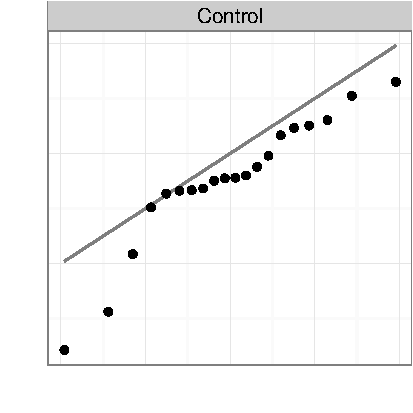
\includegraphics[width=0.22\textwidth]{figures/qqplots-1}
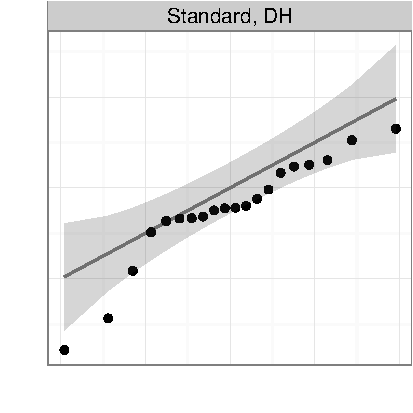
\includegraphics[width=0.22\textwidth]{figures/qqplots-2}
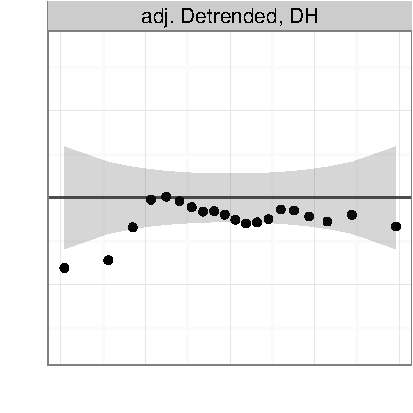
\includegraphics[width=0.22\textwidth]{figures/qqplots-3}
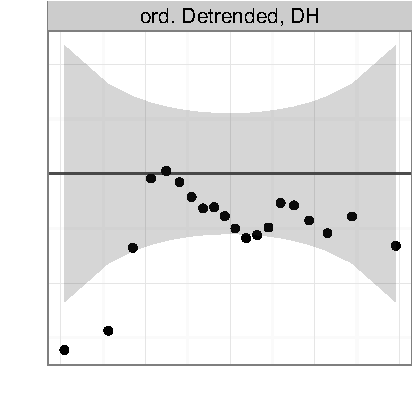
\includegraphics[width=0.22\textwidth]{figures/qqplots-4}

\includegraphics[width=0.22\textwidth]{figures/blank}
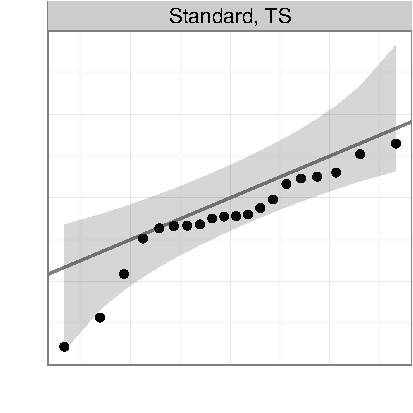
\includegraphics[width=0.22\textwidth]{figures/qqplots-5}
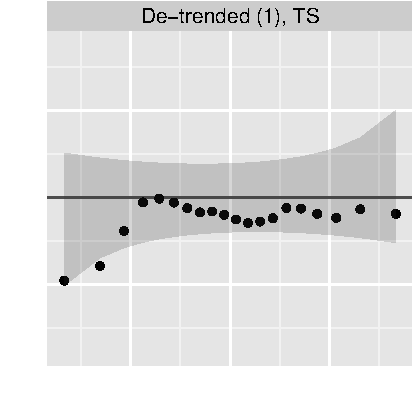
\includegraphics[width=0.22\textwidth]{figures/qqplots-6}
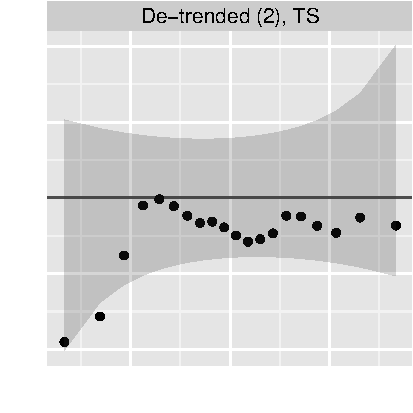
\includegraphics[width=0.22\textwidth]{figures/qqplots-7}
\caption{ \label{qqplots} \hh{Q-Q plot variations:} control, standard, and \hh{two versions of} de-trended \hh{Q-Q plots}, with Davison Hinkley (DH) or tail-sensitive (TS) 95\% confidence regions.}
\end{figure}
\afterpage{\clearpage}


In order to objectively evaluate  the three designs and quantify their effectiveness we make use of {\it lineup tests}.

\subsection{Lineup Tests}
Lineup tests have been introduced by \citet{buja:2009hp} to evaluate and quantify the significance of graphical findings. The idea behind a lineup test is that of a police lineup: the chart of the observed data is placed randomly among a set of so-called \emph{null charts}, showing data created consistently with the null hypothesis. In the setting of a lineup of normal Q-Q plots, the null hypothesis  is either that $F$ is standard normal or that $F$ is normal with parameters based on sample mean and variance.
If the `suspect'---i.e., the plot of the observed data---can be identified from the null charts, this counts as evidence against the null hypothesis. Multiple identifications of the data by independent observers then lead to a rejection of the null hypothesis. 
The lineup protocol also allows for an assessment of the power of a lineup \citep{mahbub:2013},  
%as the probability that in $N$ independent evaluations observers 
and by showing different renderings of the same data in lineups we can evaluate the power  of different designs \citep{Hofmann:2012ts}.

In considering the power of a lineup, we need to estimate the probability, $p_i$, that observer $i$ identifies the data from the lineup. If the observer is just guessing, this probability is $1/m$, where $m$ is the number of plots in the lineup.
The power of a lineup is then given as the probability to reject the null hypothesis. Let $Y$ be the number of identifications of the data plot in $N$ independent evaluations, and let $Y \sim F_N$. The power of the lineup is then the probability that more than $y_\alpha$ out of $N$ observers
choose the true plot, or more formally
\begin{equation}\label{eqn:power}
\widehat{\text{Power}} = \text{Power}_{N} = 1 - F_{Y} (y_{\alpha}),
\end{equation}
where $y_\alpha$ is the critical value for a given significance level $\alpha$, i.e.~$P(Y >  y_{\alpha}) \le \alpha$. $Y$ is composed of the sum of $N$ observers' (binary) decisions $Y_i \sim B_{1, p_i}$, where  $p_i$ is the probability that individual $i$ chooses the data plot. This probability  depends both on the strength of the signal in the data plot and an individual's visual ability.
Assessing this ability requires that each individual evaluates multiple lineups. 
If that is not possible, we must assume that all participants share the same ability, $p$. %, and the power calculation in Equation~\ref{eqn:power} simplifies to $1 - B_{N, \hat{p}}(x_\alpha)$, where $\widehat{p}$ is an estimate for the probability of choosing the data plot for a specific lineup.
Similar to classical inference, we can make use of power to assess the sensitivity of tests. This allows us to make decisions about designs for particular tasks by evaluating lineups displaying  the same data in different types of displays \citep{Hofmann:2012ts}. 


%In the next section, we describe the simulation study used to compare the three \al{(four??)} Q-Q plot designs, and an initial comparison of the three designs is given. 
\al{In Section~\ref{sec:power2} we compare the power of the lineup test of normality to the classical normality tests
 \hh{based on a simulation study, which we introduce in section~\ref{sec:simu}}. We use a generalized linear mixed model to compare the power of different designs  of Q-Q plots in Section~\ref{sec:power1}, and also explore the feedback of the independent observers to compare the rationale for plot selection (i.e.\ rejection of normality). We conclude with a discussion and outline areas for future research.}
% We use a generalized linear mixed model to compare the power of the three designs in Section~\ref{sec:power1}, and also explore the feedback of the independent observers to compare the rationale for plot selection (i.e., rejection of normality). Finally, we compare the power of a lineup test of normality to the classical normality tests in Section~\ref{sec:power2}, and outline areas for future research in Section~\ref{sec:discussion}. 


%------------------------------------------------------------------------------------
%------------------------------------------------------------------------------------

%------------------------------------------------------------------------------------
\section{Simulation Setup and Model}\label{sec:simu}
%------------------------------------------------------------------------------------

\hh{In order to evaluate the power of Q-Q plots and compare their performance to normal distribution tests, we make use of a simulation study, 
using samples of size $n \in \{20, 30, 50, 75\}$ from a $t_{d}$ distribution with $d \in \{2, 5, 10\}$ degrees of freedom. For each of these parameters we take two samples, resulting in a total of 24 samples.}
\alnote{I think using $n$ for sample size is most logical, though this does complicate the notation used in model (2).}

\hh{For the visual evaluation, we make use of Q-Q plots in a lineup test: each sample is randomly inserted among a set of 19 null plots constructed from samples of the same size drawn from the normal distribution. For each  sample, two sets of null plots are created, so that we have a total of 48 lineup \hh{data sets}. 
These lineup \hh{data sets} are rendered in each of the Q-Q plot variations, resulting in $48 \times 7 = 336$ different lineups.  Additionally, standard plots (both TS and DH bands) are rendered against $N(0, S^2)$ null data (see discussion below), adding another $2 \times 48 = 96$ lineups.
}


%To further develop the assessment of normality using lineups, we conducted a study comparing the three different versions of the Q-Q plot.
%We are testing three different versions of a Q-Q plot, 


%To investigate the power of the three different Q-Q plot versions, we sampled data from a $t$ distribution with varying degrees of freedom and sample sizes, and included a Q-Q plot of these data in a lineup of null charts drawn from standard normal samples of the same size.
For lineup tests it is extremely important to consider the generation of the null sets and the construction of the plots in the lineup. 
Null data sets must be created conistently with the null hypothesis. Here, we have two different null hypotheses to consider:

\begin{itemize}
\item{\bf Situation I:}
$H_0: F = N(0,1)$  \\
Null samples are drawn from a standard normal distribution; the reference line is the line of identity. Lines and envelopes are the same across all panels, in particular, all panels have the same scale. 
\item{\bf Situation II:} $H_0: F = N(0,S^2)$ \\
$S$ is based on the interquartile range of the data; null samples are drawn from $N(0, S^2)$. \\
The reference line has a slope of $S$ (and an intercept of 0).  All panels have the same scale. 
\end{itemize}

%\alnote{The generation of the null data makes sense to me, but is there a way to use bullet points on the right side of the table? That would help me read it...}

Examples for both \al{null} hypotheses are shown in Figure~\ref{fig:lps}. Both lineups show identical data, the sample\footnote{The little piece of calculus is imposing a small cognitive barrier that allows the reader to evaluate the lineup once without already being biased by knowing the location of the data panel.} is in panel \#$(3^2-3)$. On the left the observed data stand out (all 33 observers picked the data plot); thus, we reject the null hypothesis of a standard normal distribution. On the right, the observed data do not stand out (only 3 out of 27 observers picked the data); thus, we do not reject the null hypothesis of a normal distribution with parameters $\mu=0$ and $\widehat{S}=1.578$. \hhnote{checked the number - it's fine}
\alnote{We need to straighten out our notation for the standard deviation. On this page we use both $\widehat{\sigma}$ and $\widehat{S}$.}
\hhnote{XXX $\widehat{\sigma}$ and $\widehat{S}$ are supposed to be two different estimators -- I'm thinking of $\hat{\sigma} = 1/(n-1) \sum_i (x_i - \bar{x})^2$ whereas $\hat{S}$ is a more robust estimator based on the ratio of IQRs in y and x. We need to say that somewhere. }

\begin{figure}[hbt]

\begin{subfigure}{0.5\textwidth}
\begin{knitrout}
\definecolor{shadecolor}{rgb}{0.969, 0.969, 0.969}\color{fgcolor}
\includegraphics[width=\maxwidth]{figure/unnamed-chunk-1-1} 

\end{knitrout}
\end{subfigure}
\begin{subfigure}{0.5\textwidth}
\begin{knitrout}
\definecolor{shadecolor}{rgb}{0.969, 0.969, 0.969}\color{fgcolor}
\includegraphics[width=\maxwidth]{figure/unnamed-chunk-2-1} 

\end{knitrout}
\end{subfigure}
\caption{\label{fig:lps} Lineup plots of standard Q-Q plots. The observed data is the same, but  reference lines and envelopes are based on a standard normal distribution on the left; while  reference lines and envelopes for the lineup on the right are based on a normal distribution $N(0, \widehat{S}^2)$, where $\widehat{S}$ is based on the IQR of the observed data.
The observed data plot in both lineups is displayed in panel \#$(3^2 - 3)$. }
\end{figure}
\afterpage{\clearpage}

Note that the above list of hypotheses is not exhaustive. Any theoretical distribution in a Q-Q plot corresponds to a  hypothesis test against that distribution, and as long as there is a method to generate samples under the null hypothesis, we do not even need to know the exact distribution. This allows us to assess situations in which we only have approximate or asymptotic results, which are otherwise hard, if not impossible, to investigate  with the (small) finite samples we typically deal with in practice.
\al{Additionally, we use the interquartile range (IQR) to estimate scale, as it is a standard practice for Q-Q plots.}

\hhnote{`as it is a standard practice' is not stating quite the same as what I was trying to say before. I was not trying to give a reason for why we use a robust estimate, but just stating that this estimator is standard practice for Q-Q plots. 
How about 

``Additionally, we use the interquartile range (IQR) to estimate scale, as is standard practice for Q-Q plots."
}
% The interquartile range (IQR) is used---as is standard practice for Q-Q plots---to estimate scale. 
Robust estimation of the variance is preferred for better assessment of the tails and outliers of the empirical distribution. We could use alternative estimators for variance, such as median absolute deviation (MAD) or adjusted MAD \citep{rousseeuw}, but this will likely also change the power of the corresponding lineup.

Using  Amazon MTurk \citep{amazon}, 1369 independent observers were recruited and asked to evaluate ten lineups each. \hh{Lineups were randomly assigned to participants, such that each participant
(i) evaluated each data set at most once, 
(ii) was exposed to multiple parameter settings (`harder' and `easier' lineups), and
(iii) evaluated each Q-Q plot design at most twice.

\alnote{I can do this soon.}
XXX discussion of amazon turk studies in comparison to lab experiments: practical considerations \citep{Kosara:2010}, study by \citet{cleveland:1984} re-run on Amazon MTurk with similar results by \citet{Heer:2010}.
}
%
Half of the lineups that observers were shown allowed for multiple choices of plots from a lineup for the final answer. Very few participants made use of this option. In the analysis we dealt with multiple answers to a lineup by using a weighting variable defined as the reciprocal of the number of answers given by a participant.





\begin{figure}[ht]
\centering






























